% Lecture Template for ME3001 - Mechanical Engineering Analysis - Tennessee Technological University
% Spring 2024 - condensing and streamlining lectures by combining topics into a single PDF under the module name
% this will simplify file and link management as well as make lectures easier to use in class
% - added image/ to clean directory and reduce redundancy, specific to module for now  

% Module Name: Ordinary Differential Equations
% Topic 1 - Review and Classification
% Topic 2 - Analytical Solution Techniques 
% Topic 3 - Numerical Solution Techniques
% Topic 4 - ...

\documentclass[fleqn]{beamer} % for presentation (has nav buttons at bottom)

\usepackage{../analysis_lectures}

\author{ME3001 - Mechanical Engineering Analysis}

\newcommand{\MNUM}{4\hspace{2mm}} % module number 
\newcommand{\moduletitle}{Ordinary Differential Equations}

\newcommand{\sectionItitle}{Review and Classification}
\newcommand{\sectionIItitle}{Analytical Solution Techniques}
\newcommand{\sectionIIItitle}{Numerical Solution Techniques}
\newcommand{\sectionIVtitle}{...}

\newcommand{\sectionIsubsectionItitle}{What is a Differential Equation?}
\newcommand{\sectionIsubsectionIItitle}{Standard Form of an ODE}
\newcommand{\sectionIsubsectionIIItitle}{Classification}
\newcommand{\sectionIsubsectionIVtitle}{Examples}

\newcommand{\sectionIIsubsectionItitle}{Analytical vs Numerical Methods}
\newcommand{\sectionIIsubsectionIItitle}{Separation of Variables}
\newcommand{\sectionIIsubsectionIIItitle}{Trial Solution Method}
\newcommand{\sectionIIsubsectionIVtitle}{Soluition Cases}

\newcommand{\sectionIIIsubsectionItitle}{Review and Motivation}
\newcommand{\sectionIIIsubsectionIItitle}{Analytical vs Numerical Methods}
\newcommand{\sectionIIIsubsectionIIItitle}{Euler's Forward Integration}
\newcommand{\sectionIIIsubsectionIVtitle}{Example Problem}
\newcommand{\sectionIIIsubsectionVtitle}{MATLAB Solution}

\newcommand{\sectionIVsubsectionItitle}{}
\newcommand{\sectionIVsubsectionIItitle}{}
\newcommand{\sectionIVsubsectionIIItitle}{}
\newcommand{\sectionIVsubsectionIVtitle}{}

\newcommand{\paramM}{100} % mass, m
\newcommand{\paramC}{0.5}  % drag coeff, c
\newcommand{\paramVO}{5.0} % initial velocity, v0
\newcommand{\paramDTA}{1.0} % timestep, dt  - A
\newcommand{\paramDTB}{0.1} % timestep, dt  - B
\newcommand{\paramDTC}{0.01} % timestep, dt  - C


% custom box
\newsavebox{\mybox}

\title{Lecture Module - \moduletitle}

\date{Mechanical Engineering\vspc Tennessee Technological University}

\begin{document}

	\lstset{language=MATLAB,basicstyle=\ttfamily\small,showstringspaces=false}

	\frame{\titlepage \center\begin{framed}\Large \textbf{Module \MNUM - \moduletitle}\end{framed} \vspace{5mm}}

	% Module Outline
	\begin{frame} 
		\large \textbf{Module \MNUM - \moduletitle} \vspace{3mm}\\

		\begin{itemize}
			\item Topic 1 - \hyperlink{sectionI}{\sectionItitle} \vspc % section I
			\item Topic 2 - \hyperlink{sectionII}{\sectionIItitle} \vspc % section II
			\item Topic 3 - \hyperlink{sectionIII}{\sectionIIItitle} \vspc % section III
			\item Topic 4 - \hyperlink{sectionIV}{\sectionIVtitle} \vspc % section IV
		\end{itemize}

	\end{frame}

	% section I
	\section{\sectionItitle}\label{sectionI}

		% section I Outline
		\begin{frame} 
			\large \textbf{Topic 1 - \sectionItitle} \vspace{3mm}\\

			\begin{itemize}
				\item \hyperlink{sectionIsubsectionI}{\sectionIsubsectionItitle} \vspc %  section I subsection I
				\item \hyperlink{sectionIsubsectionII}{\sectionIsubsectionIItitle} \vspc % section I subsection II
				\item \hyperlink{sectionIsubsectionIII}{\sectionIsubsectionIIItitle} \vspc % section I subsection III
				\item \hyperlink{sectionIsubsectionIV}{\sectionIsubsectionIVtitle} \vspc % section I subsection IV
			\end{itemize}
		\end{frame}
	

		% section I subsection I 
		\subsection{\sectionIsubsectionItitle}\label{sectionIsubsectionI}

			\begin{frame}
				\frametitle{\sectionIsubsectionItitle}
				\bigskip

				\frametitle{What is a Differential Equation?}
				  {\it Definition:\vspace{3mm}\\}
				  A {\bf differential equation} is an equation which describes a function \vspace{3mm}\\and one or more of its \underline{\hspace{50mm}} of the \vspace{3mm}\\ \underline{\hspace{50mm}}\hspace{3mm}\underline{\hspace{50mm}}\vspace{5mm} \\ with respect to the \underline{\hspace{60mm}}.

				
				\btVFill
			\end{frame}

			% \begin{frame}
			% 	\frametitle{\sectionIsubsectionItitle}
			% 	\bigskip

				
			% 	\btVFill
			% \end{frame}


		% section I subsection II
		\subsection{\sectionIsubsectionIItitle}\label{sectionIsubsectionII}

			\begin{frame}
				\frametitle{\sectionIsubsectionIItitle} \small
				\bigskip

				  Ordinary Differential Equations are written in the following form.\vspace{3mm}\\

\scalebox{1.2}{$a_n\frac{dy^{(n)}}{d^{(n)}x}+a_{n-1}\frac{dy^{(n-1)}}{d^{(n-1)}x}+...+a_{2}\frac{dy^{2}}{d^{2}x}+a_{1}\frac{dy}{dx}+a_0y=f(x)$}	\vspace{0mm}\\		

The apostrophe is commonly used for the derivative. \vspace{2mm}\\

\scalebox{1.2}{$a_ny^{(n)}+a_{n-1}y^{(n-1)}+...+a_2y'' +a_1y'+a_0y=f(x)$} \vspace{3mm}\\

If time is the independent variable the equation changes slightly. \vspace{2mm}\\

				
				\btVFill
			\end{frame}


		% section I subsection III
		\subsection{\sectionIsubsectionIIItitle}\label{sectionIsubsectionIII}
			\begin{frame} 
				\frametitle{\sectionIsubsectionIIItitle}
				\bigskip

				\frametitle{Is the differential equation ordinary or partial?}

An {\bf ordinary} differential equation has \underline{\hspace{20mm}} independent \vspc variable and \underline{\hspace{20mm}} dependent variable. \vspace{10mm}\\

A {\bf partial} differential equation has \underline{\hspace{50mm}} \vspc independent variable  \underline{\hspace{20mm}}  dependent variable. \vspace{10mm}\\

				
				\btVFill
			\end{frame}	

			\begin{frame} 
				\frametitle{\sectionIsubsectionIIItitle}
				\bigskip

				\frametitle{What is the order of the equation?}
  
The {\bf order} of a differential equation is the \vspace{3mm}\\ \underline{\hspace{50mm}}\hspace{3mm}\underline{\hspace{50mm}} \vspace{5mm}\\ present in the equation. \vspace{3mm}\\	

			 
				\btVFill
			\end{frame}	

			\begin{frame} 
				\frametitle{\sectionIsubsectionIIItitle}
				\bigskip

				  \frametitle{What is the degree of the equation?}

The {\bf degree} of a differential equation is the \underline{\hspace{30mm}}\hspace{3mm} \vspace{5mm}\\ of its highest derivative, after the equation has been made rational \vspace{5mm}\\ and integral in all of its derivatives. \vspace{3mm}\\

			 
				\btVFill
			\end{frame}	

			\begin{frame} 
				\frametitle{\sectionIsubsectionIIItitle}
				\bigskip

				\frametitle{Is the differential equation linear or non-linear?}

An ordinary differential equation is \underline{\hspace{30mm}} if the following statements are true. \vspace{5mm}\\

\begin{enumerate}
\item {\it The dependent variable and its derivatives are of the first degree.} \vspace{3mm}\\

\item {\it The coefficients are constants or dependent on the independent variable.}\vspace{3mm}\\
\end{enumerate}

If either rule is broken, the equation is \underline{\hspace{10mm}}-\underline{\hspace{30mm}}.

			 
				\btVFill
			\end{frame}	



		% section I subsection IV
		\subsection{\sectionIsubsectionIVtitle}\label{sectionIsubsectionIV}	

			\begin{frame}
				\frametitle{\sectionIsubsectionIVtitle}
				\bigskip


Differential equations are used to describe physical systems in many areas of engineering. An equation that represents a physical (or theoretical) system is known as a \underline{\hspace{50mm}}\hspace{3mm}\underline{\hspace{50mm}}.\vspace{3mm}\\
\begin{itemize}

	\item Solid Mechanics \vspace{3mm}\\
	\item Kinematics and Dynamics \vspace{3mm}\\
	\item Heat Transfer and Thermodynamics \vspace{3mm}\\
	\item Fluid Mechanics
			
\end{itemize}


				\btVFill
			\end{frame}
	
			\begin{frame}
				\frametitle{\sectionIsubsectionIVtitle}
				\bigskip

				\begin {multicols}{2}

Newton's Second Law \vspace{2mm}\\

$\Sigma {\bf F}=m {\bf a}$ \vspace{2mm}\\

leads  to an {\it equation of motion}.  \vspace{2mm}\\

$\dot{y}+\frac{c}{m}y=f(t)$

 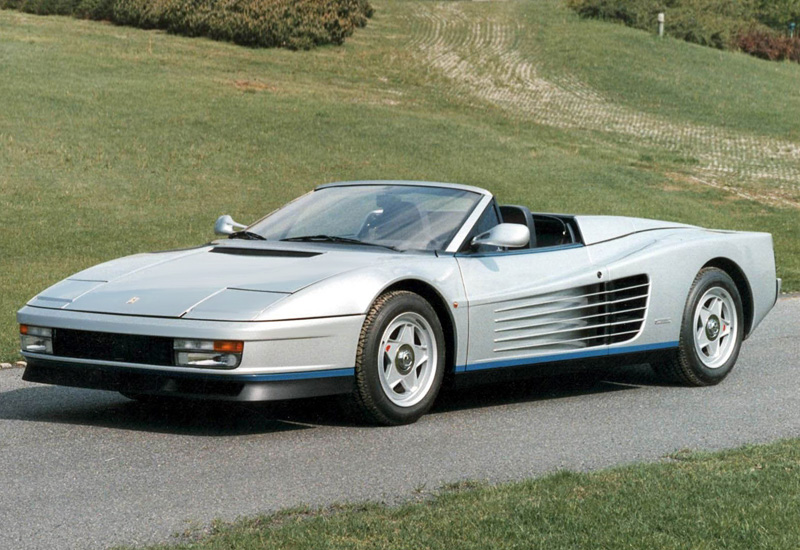
\includegraphics[scale=0.15]{images/ferrari.jpg}\\
 
 \end{multicols} 


				\btVFill
			\end{frame}


 			\begin{frame}
 				\frametitle{\sectionIsubsectionIVtitle}
 				\bigskip

				\begin {multicols}{2}

The {\bf solution} to a differential equation describes the \vspace{2mm}\\ \underline{\hspace{40mm}}\hspace{2mm}\underline{\hspace{40mm}} as a function \vspace{2mm}\\of the \underline{\hspace{40mm}}\hspace{2mm}\underline{\hspace{40mm}}.  \vspace{5mm}\\


	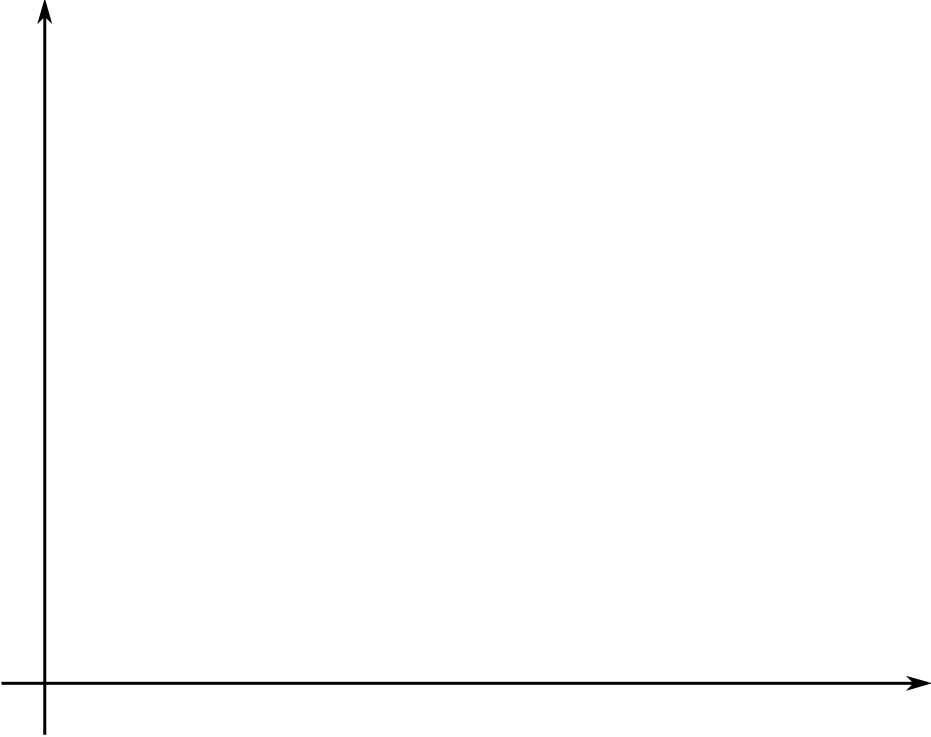
\includegraphics[scale=0.10]{images/lecture1_fig2.png} \hspace{10mm} 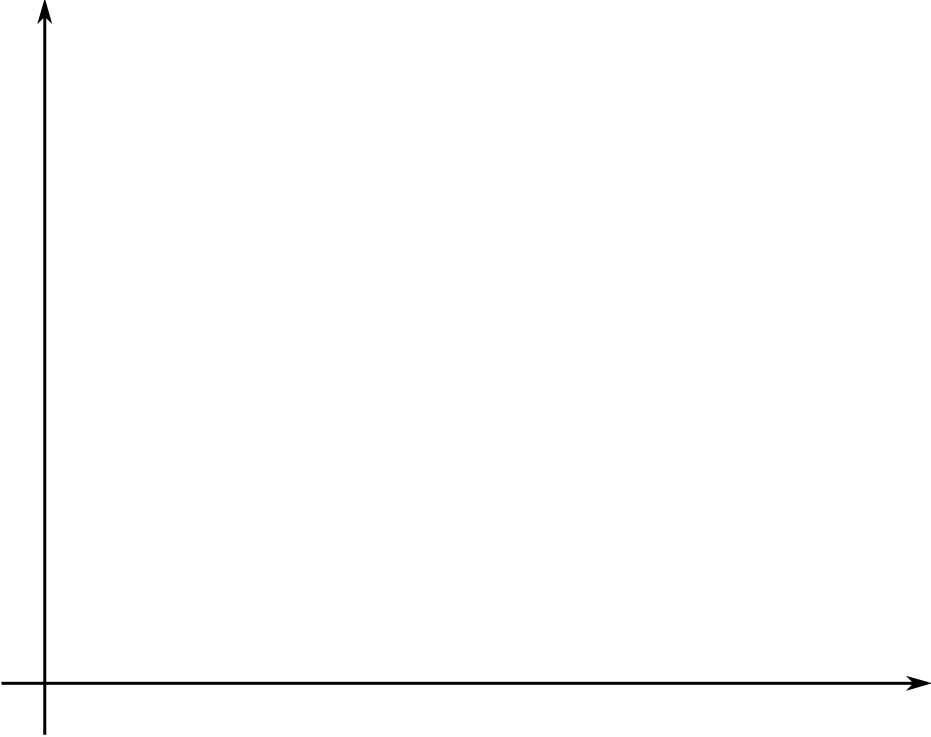
\includegraphics[scale=0.10]{images/lecture1_fig2.png}\vspace{2mm}\\
	
	%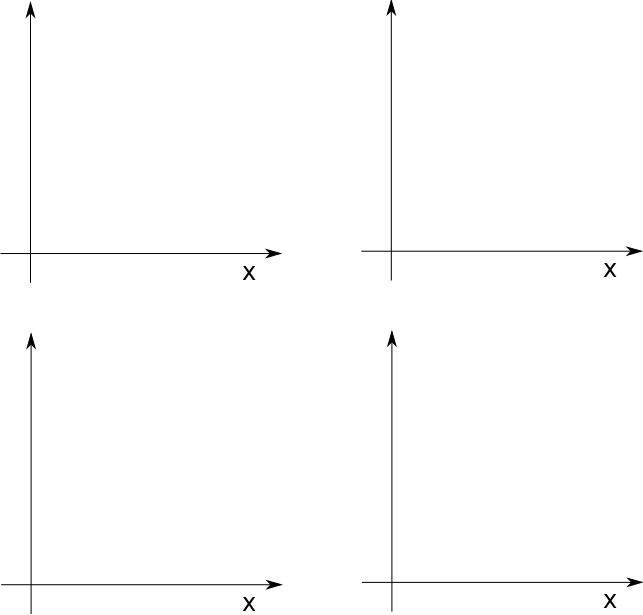
\includegraphics[scale=0.1]{lecture1_fig2.png}\\	
	
There are many different methods for finding the solution.

\end{multicols} 
 				\btVFill
			\end{frame}


	% Section II
	\section{\sectionIItitle}\label{sectionII}

		% section II Outline
		\begin{frame}
			\large \textbf{Topic 2 - \sectionIItitle} \vspace{3mm}\\

			\begin{itemize}
				\item \hyperlink{sectionIIsubsectionI}{\sectionIIsubsectionItitle} \vspc %  section II subsection I
				\item \hyperlink{sectionIIsubsectionII}{\sectionIIsubsectionIItitle} \vspc % section II subsection II
				\item \hyperlink{sectionIIsubsectionIII}{\sectionIIsubsectionIIItitle} \vspc % section II subsection III
				\item \hyperlink{sectionIIsubsectionIV}{\sectionIIsubsectionIVtitle} \vspc % section II 
			\end{itemize}

		\end{frame}

		% section II subsection I
		\subsection{\sectionIIsubsectionItitle}\label{sectionIIsubsectionI}

			\begin{frame}[label=sectionIIsubsectionI]
				\frametitle{\sectionIIsubsectionItitle}
				\bigskip

  
				\btVFill
			\end{frame}

			\begin{frame}[label=sectionIIsubsectionI]
				\frametitle{\sectionIIsubsectionItitle}
				\bigskip


				\btVFill
			\end{frame}	

			\begin{frame}[label=sectionIIsubsectionI]
				\frametitle{\sectionIIsubsectionItitle}
				\bigskip

				
				\btVFill
			\end{frame}

		% section II subsection II
		\subsection{\sectionIIsubsectionIItitle}\label{sectionIIsubsectionII}

			\begin{frame}
				\frametitle{\sectionIIsubsectionIItitle} \small
				\bigskip


				\btVFill 
			\end{frame}	

			\begin{frame}
				\frametitle{\sectionIIsubsectionIItitle} \small
				\bigskip


				\btVFill
			\end{frame}		


		% section II subsection III
		\subsection{\sectionIIsubsectionIIItitle}\label{sectionIIsubsectionIII}

			\begin{frame}
				\frametitle{\sectionIIsubsectionIIItitle} \small
				\bigskip

				
				\btVFill 
			\end{frame}

			\begin{frame}
				\frametitle{\sectionIIsubsectionIIItitle}\small
				\bigskip


				\btVFill 
			\end{frame}


		% section II subsection IV 
		\subsection{\sectionIIsubsectionIVtitle}\label{sectionIIsubsectionIV}

			\begin{frame}
				\frametitle{\sectionIIsubsectionIVtitle}
				\bigskip

				
				\btVFill 
			\end{frame}

			\begin{frame}
				\frametitle{\sectionIIsubsectionIVtitle}
				\bigskip


				\btVFill 
			\end{frame}
		

	% Section III
	\section{\sectionIIItitle}\label{sectionIII}

		% section III Outline
		\begin{frame}
			\large \textbf{Topic 3 - \sectionIIItitle} \vspace{3mm}\\

			\begin{itemize}
				\item \hyperlink{sectionIIIsubsectionI}{\sectionIIIsubsectionItitle} \vspc %  section III subsection I
				\item \hyperlink{sectionIIIsubsectionII}{\sectionIIIsubsectionIItitle} \vspc % section III subsection II
				\item \hyperlink{sectionIIIsubsectionIII}{\sectionIIIsubsectionIIItitle} \vspc % section III subsection III
				\item \hyperlink{sectionIIIsubsectionIV}{\sectionIIIsubsectionIVtitle} \vspc % section III subsection IV
			\end{itemize}

		\end{frame}


		% section III subsection I
		\subsection{\sectionIIIsubsectionItitle}\label{sectionIIIsubsectionI}

			\begin{frame}
				\frametitle{\sectionIIIsubsectionItitle}
				\bigskip

				  	\frametitle{What is a Differential Equation? Solution?}

					A {\bf differential equation} is an equation which describes a function \vspace{3mm}\\and one or more of its \underline{\hspace{50mm}} of the \vspace{3mm}\\ \underline{\hspace{50mm}}\hspace{3mm}\underline{\hspace{50mm}}\vspace{2mm}\\ with respect to the \underline{\hspace{60mm}}. \vspace{8mm} \\
					 
					The {\bf solution} to a differential equation describes the \vspace{2mm}\\ \underline{\hspace{40mm}}\hspace{2mm}\underline{\hspace{40mm}} as a function \vspace{2mm}\\of the \underline{\hspace{40mm}}\hspace{2mm}\underline{\hspace{40mm}}.  \vspace{5mm}\\

			  	
				\btVFill
			\end{frame}

			\begin{frame}
				\frametitle{\sectionIIIsubsectionItitle}
				\bigskip

			  
				\btVFill
			\end{frame}


		% section III subsection II
		\subsection{\sectionIIIsubsectionIItitle}\label{sectionIIIsubsectionII}	

			\begin{frame}
				\frametitle{\sectionIIIsubsectionIItitle}
				\bigskip

				\frametitle{Analytical vs. Numerical Solutions}

				\textbf{Analytical}
				\begin{itemize}
					\item solution to a problem that can be written in {\bf closed form} 
					\item solution in terms of known functions, constants, etc.  
					\item gives an {\bf exact answer}  \vspcc
				\end{itemize}

				\textbf{Numerical}
				\begin{itemize}
					\item an {\bf approximation} to the solution of a mathematical equation
					\item known as {\bf numerical integration}
					\item numerical integration is more than {\it the computation of integrals}
				\end{itemize}
				
				\btVFill
			\end{frame}

			\begin{frame}
				\frametitle{\sectionIIIsubsectionIItitle}
				\bigskip
				\frametitle{Which one should you choose?}

				\scalebox{2}{?\hspc?\hspc?\hspc?\hspc?} \vspcc
				 
				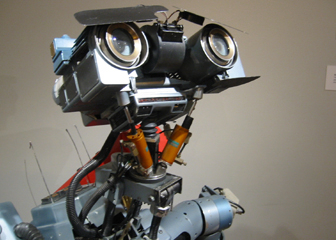
\includegraphics[scale=.3]{images/johnny5_01.jpg}\vspcc
				\scalebox{1.25}{It depends on the problem. It also depends on} \vspc
				\scalebox{1.25}{how you intend to use the solution.} \vspcc
								

				\btVFill
			\end{frame}


		% section III subsection III
		\subsection{\sectionIIIsubsectionIIItitle}\label{sectionIIIsubsectionIII}

			\begin{frame}
				\frametitle{\sectionIIIsubsectionIIItitle}
				\bigskip

				\frametitle{The Initial Value Problem}

				You learned about the {\bf initial value problem} in differential equations class. Do you remember?\vspcc

				You have probably been thinking about this idea for much longer than that. Consider riding in a {\it truck} waiting to arrive at you destination...\vspace{10mm}\\
				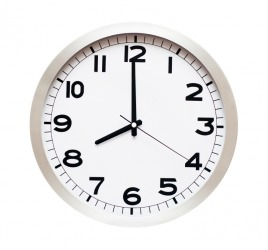
\includegraphics[scale=0.15]{images/time.jpg}\\
				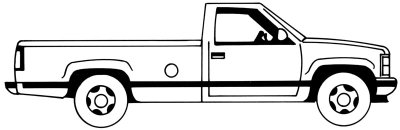
\includegraphics[scale=0.35]{images/lecture1_fig1_1.png}

				\btVFill
			\end{frame}

			\begin{frame}
				\frametitle{\sectionIIIsubsectionIIItitle}
				\bigskip

				\frametitle{Integrating a Rate}

You may not have known it but you where {\bf integrating} when performing these mental calculations. You can math.\vspace{20mm}\\

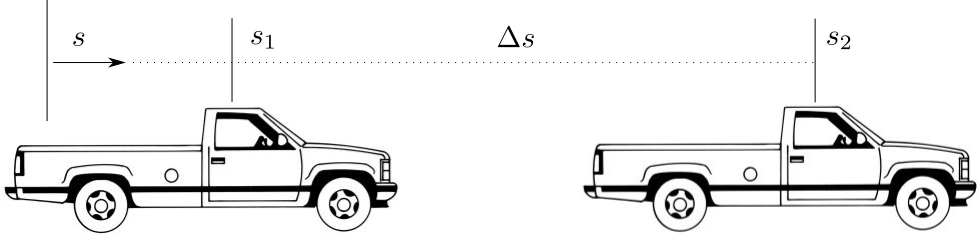
\includegraphics[scale=0.35]{images/lecture1_fig2_1.png}


				\btVFill
			\end{frame}


		% section III subsection IV
		\subsection{\sectionIIIsubsectionIVtitle}\label{sectionIIIsubsectionIV}

			\begin{frame}
				\frametitle{\sectionIIIsubsectionIVtitle}
				\bigskip

				\begin{multicols}{2}
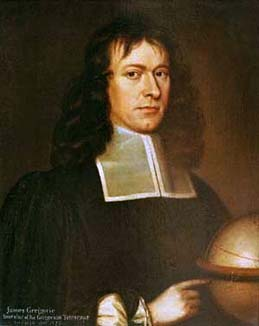
\includegraphics[scale=0.2]{images/James_Gregory.jpeg}\vspc
\small James Gregory (1638-1675)

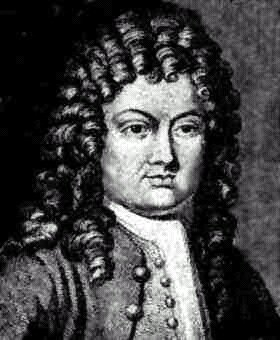
\includegraphics[scale=0.2]{images/BTaylor.jpg}\vspc
\small Brook  Taylor (1685-1731)
\end{multicols}

\frametitle{The Taylor Series}


Consider the Taylor Series. How does this apply to our problem? \vspc
\scalebox{1}{$y(x)\approx$}\vspc
\scalebox{.9}{$y(a)+y'(a)(x-a)+\frac{y''(a)}{2!}(x-a)^2+\frac{y^{(3)}(a)}{3!}(x-a)^3+...+\frac{y^{(n)}(a)}{n!}(x-a)^n$}\vspc
What does this even mean?


				\btVFill
			\end{frame}	

			\begin{frame}
				\frametitle{\sectionIIIsubsectionIVtitle}
				\bigskip

				\frametitle{Euler's Method}

Given a {\it function describing the slope} and an {\it initial condition}, discretized values of the solution can be approximated. \vspc
This is known as {\bf Euler's method}.\vspccc

	\scalebox{1.0}{$y(x+\Delta x)=y(x) + \frac{dy}{dx}\Delta x=y(x) + f(x,y(x))\Delta x$}\vspcc
	It is commonly shown with subscript notation.\\
	
	\begin{framed}
	\scalebox{1.0}{$y(x_{i+1})=y(x_i) + f(x_i,y(x_i))=y_i + f(x_i,y_i)\Delta x$}\vspcc
	\end{framed}

\small Careful: This is not the same as Euler's formula which is an essential trigonometric identity also used in differential equations.\\


				\btVFill
			\end{frame}	

			\begin{frame}
				\frametitle{\sectionIIIsubsectionIVtitle}
				\bigskip

				\frametitle{The Slope Function}

The differential equation must be written as a function describing the first derivative or {\bf the slope} of the dependent variable.\vspc

	\scalebox{1.25}{$f(x,y)=\frac{rise}{run}=\frac{dy}{dx}\neq y(x)$}\vspcc
	or with subscript notation shown below\vspcc
	\scalebox{1.25}{$f(x_i,y_i)$}\vspcc
	

\small Careful: The first argument $x$ is not always used and is often left out. However it is an important placeholder (ODE45()) and shows this method can be used for {\it non-linear} equations with generalized input functions. 


				\btVFill
			\end{frame}	

			\begin{frame}
				\frametitle{\sectionIIIsubsectionIVtitle} \small
				\bigskip

				\frametitle{Forward Integration}

Using this concept to solve the initial value problem is called {\bf Euler's forward integration} or {\bf Euler's Method}. Most of the time, the independent variable is \underline{\hspace{30mm}}. \vspcc

Compute the values of the solution one-by-one {\bf forward in time}. \vspcc
\begin{multicols}{2}
\scalebox{1}{$\underline{y(t_{i+1})=y(t_i)+f(t_i,y_i)\Delta t}$}\vspc
\scalebox{1}{$y(\hspccc)=y(\hspccc)+f(\hspccc,\hspccc)\Delta t$}\vspc
\scalebox{1}{$y(\hspccc)=y(\hspccc)+f(\hspccc,\hspccc)\Delta t$}\vspc
\scalebox{1}{$y(\hspccc)=y(\hspccc)+f(\hspccc,\hspccc)\Delta t$}\vspc

\hspace{5mm}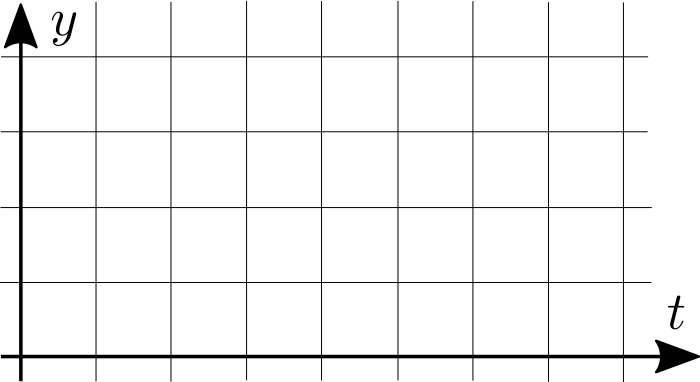
\includegraphics[scale=0.25]{images/lecture1_fig3_1.png}
\end{multicols}


				\btVFill
			\end{frame}	

	
	% Section IV
	\section{\sectionIVtitle}\label{sectionIV}

		% section IV Outline
		\begin{frame}
			\large \textbf{Topic 3 - \sectionIVtitle} \vspace{3mm}\\

			\begin{itemize}
				\item \hyperlink{sectionIVsubsectionI}{\sectionIVsubsectionItitle} \vspc %  section IV subsection I
				\item \hyperlink{sectionIVsubsectionII}{\sectionIVsubsectionIItitle} \vspc % section IV subsection II
				\item \hyperlink{sectionIVsubsectionIII}{\sectionIVsubsectionIIItitle} \vspc % section IV subsection III
				\item \hyperlink{sectionIVsubsectionIV}{\sectionIVsubsectionIVtitle} \vspc % section IV subsection IV
			\end{itemize}

		\end{frame}

		% section IV subsection I
		\subsection{\sectionIVsubsectionItitle}\label{sectionIVsubsectionI}

			\begin{frame}
				\frametitle{\sectionIVsubsectionItitle}
				\bigskip

				\frametitle{The Previous Example - Radio Flyer}

\begin{multicols}{2}
If this is a valid technique we should be able to solve the problem we solved in the previous lecture. Ferrari anyone? Let's do a Radio Flyer instead. \\ 

\hspace{10mm}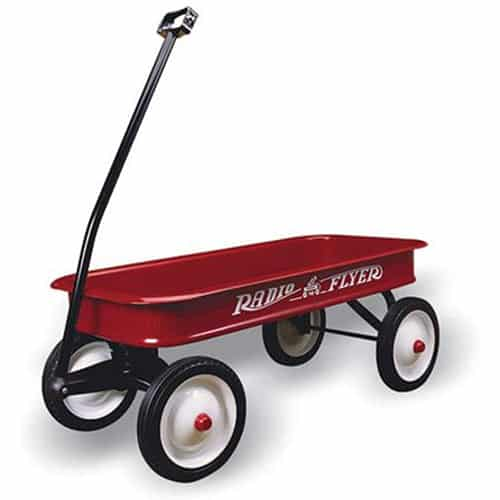
\includegraphics[scale=0.15]{images/Radio-Flyer.jpg} \vspc

\end{multicols}

\scalebox{1.25}{$m\dot{v}+cv=0 \hspace{3mm} with \hspace{3mm}v(t=0)=v_0$} \vspcc
\scalebox{1.25}{$\hspace{5mm}\implies\hspace{5mm}v(t)=v_0e^{-\frac{c}{m}t}$} \vspace{5mm}\\

		
				\btVFill
			\end{frame}

		% section IV subsection II
		\subsection{\sectionIVsubsectionIItitle}\label{sectionIVsubsectionII}

			\begin{frame}
				\frametitle{\sectionIVsubsectionIItitle}
				\bigskip

				\frametitle{The Problem Statement}

This method is not difficult {\it if} we setup  the problem correctly. Read the problem statement carefully.\vspcc

\begin{framed}
Approximate a solution to the differential equation using Euler's Method. Graph the solution from $0$ to $10$ seconds and use a stepsize of $\Delta t=\paramDTA,\hspc\paramDTA,\hspc$and$\hspc \paramDTA $ seconds.\vspcc
\scalebox{1.25}{$m\dot{v}+cv=0 \hspace{3mm} with \hspace{3mm}v(t=0)=v_0$}\vspcc
\scalebox{1.0}{$m=\paramM(kg), \hspc c=\paramC (\frac{n-m}{s}), v_0=\paramVO(\frac{m}{s})$}
\end{framed}


				\btVFill
			\end{frame}

			\begin{frame}
				\frametitle{\sectionIVsubsectionIItitle}
				\bigskip


\frametitle{Breakdown The Problem Statement}
\begin{tabular}{cc}
\underline{ODE:}&\scalebox{1.0}{$m\dot{v}+cv=0$}\vspcc
\underline{Initial Condition:}&\scalebox{1.0}{$\hspace{3mm}v(t=0)=v_0$}\vspcc
\underline{Parameters:}&\scalebox{1.0}{$m=100(kg), \hspc c=0.5 (\frac{n-m}{s}), v_0=5(\frac{m}{s})$}\vspcc
\underline{Strategy:}& Euler's Method, $\Delta t=\paramDTA,\hspc\paramDTB,\hspc$and$\hspc \paramDTC (s) $  \vspccc
\end{tabular}

Look at the formula we derived. What goes where?\vspcc


\scalebox{1.0}{$y_{i+1}=y_i + f(x_i,y_i)\Delta x$}\vspcc


				\btVFill
			\end{frame}	


		% section IV subsection III
		\subsection{\sectionIVsubsectionIIItitle}\label{sectionIVsubsectionIII}

			\begin{frame}
				\frametitle{\sectionIVsubsectionIIItitle}
				\bigskip

				\frametitle{Execute Euler's Method}
First, write the {\bf slope function}. \vspc
\scalebox{1}{$f(t,y(t))=f(t,y)=$}\vspc
Then, start with the initial condition and compute the values of the solution {\it one by one, forward in time}. \vspcc

\scalebox{1}{$\underline{v(t_{i+1})=v(t_i)+f(v(t_i))\Delta t}$}\vspc
\scalebox{1}{$v(\hspccc)=v(\hspccc)+f(\hspccc)\Delta t$}\vspc
\scalebox{1}{$v(\hspccc)=v(\hspccc)+f(\hspccc)\Delta t$}\vspc
\scalebox{1}{$v(\hspccc)=v(\hspccc)+f(\hspccc)\Delta t$}\vspc
\scalebox{1}{$v(\hspccc)=v(\hspccc)+f(\hspccc)\Delta t$}\vspc

 This method is not suitable for manual computation. \vspace{0mm}\\


				
				\btVFill
			\end{frame}	

			\begin{frame}
				\frametitle{\sectionIVsubsectionIIItitle}
				\bigskip

				
				\btVFill
			\end{frame}	


				\begin{frame}
				\frametitle{\sectionIVsubsectionIIItitle}
				\bigskip

				
				\btVFill
			\end{frame}	

				\begin{frame}
				\frametitle{\sectionIVsubsectionIIItitle}
				\bigskip

				
				\btVFill
			\end{frame}		

\end{document}





